\chapter{Thực nghiệm Sư phạm}

\section{Mục tiêu thực nghiệm}\begin{itemize}
	\item Tìm hiểu khả năng ứng dụng AI vào đánh giá năng lực của học sinh.
	\item Phân tích sự chính xác của kết quả kiểm tra thích ứng so với điểm trung bình môn Toán của học sinh, từ đó nhận xét về tính khả quan của Kant bot trong đánh giá năng lực học sinh.
	\item Cải tiến và hoàn thiện Kant bot.
\end{itemize}

\section{Đối tượng và tiến trình thực nghiệm}
\subsection{Đối tượng thực nghiệm}
	38 học sinh lớp 11, 12 thuộc các trường THPT Châu Văn Liêm, Lý Tự Trọng và Thực hành Sư phạm.

\subsection{Tiến trình thực nghiệm}
\begin{enumerate}[label=\textbf{Giai đoạn \arabic*.},align=left,left=0cm..0cm,itemindent=*]
	\item Gửi đường link truy cập cho học sinh làm thực nghiệm phần Tổ hợp – Xác suất với sự đánh giá tự động của Kant bot.\par
	\item Phân tích quá trình đánh giá của Kant đối với một số học sinh.
	\item Tổng hợp và phân tích kết quả đánh giá của học sinh.
\end{enumerate}

\section{Nội dung thực nghiệm}
Quá trình thực nghiệm chính được thực hiện hoàn toàn trực tuyến với Kant bot, thông qua nền tảng Facebook Messenger.\par
Trong phần này, người dùng cần phải thực hiện tối đa 10 CH trắc nghiệm\cite{le2015xay} cho một chủ đề – với CH được đưa ra dựa trên dữ liệu trả lời những câu hỏi trước – để đạt tới mức kỳ vọng ổn định nhất (dưới $0.8$). Sau đó Kant sẽ đưa ra kết quả đánh giá năng lực. Hình \ref{fig:fig-c4-chatbot-demo} minh họa quá trình thực nghiệm đánh giá với Kant.
\begin{figure}[htb!]\centering
	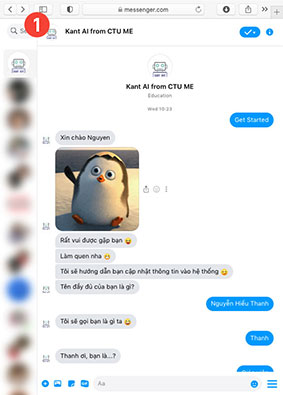
\includegraphics[width=7cm]{kant-ux/chat-1}
	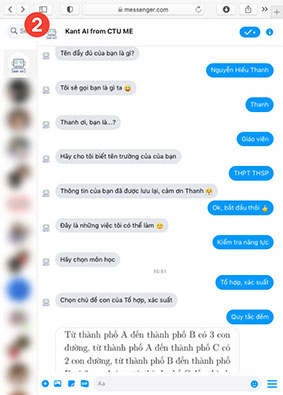
\includegraphics[width=7cm]{kant-ux/chat-2}
	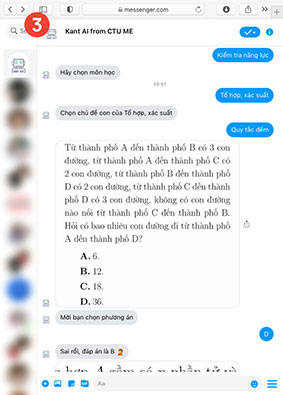
\includegraphics[width=7cm]{kant-ux/chat-3}
	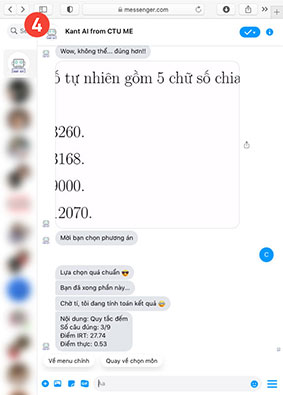
\includegraphics[width=7cm]{kant-ux/chat-4}
	\caption{Minh họa quá trình thực nghiệm với Kant}
	\label{fig:fig-c4-chatbot-demo}
\end{figure}\par

\section{Kết quả thực nghiệm}

Có 38 học sinh hoàn thành phần kiểm tra năng lực chương Tổ hợp, xác suất. Kết quả đánh giá năng lực bằng Kant bot được tổng hợp ở bảng \ref{tab:tab-s4-result}, danh sách được sắp xếp và đặt mã số theo \textit{Sai số} giảm dần.

\begin{longtable}{ScSlScScScSc}
	\caption{Kết quả thực nghiệm đánh giá bằng Kant bot}\label{tab:tab-s4-result}\\
	\textbf{TT} & \multicolumn{1}{Sc}{\textbf{Trường THPT}} & \textbf{Lớp} & \textbf{KQ đánh giá} & \textbf{ĐTB Toán} & \textbf{Sai số} \\ \hline\endfirsthead

	\textbf{TT} & \multicolumn{1}{Sc}{\textbf{Trường THPT}} & \textbf{Lớp} & \textbf{KQ đánh giá} & \textbf{ĐTB Toán} & \textbf{Sai số} \\ \hline\endhead\hline\endfoot

	S01 & Châu Văn Liêm     & 11 & $9.7$ & $9.7$ & $0.0$ \\

	S02 & Thực hành Sư phạm & 11 & $8.8$ & $8.7$ & $0.1$ \\
	S03 & Thực hành Sư phạm & 11 & $8.4$ & $8.5$ & $0.1$ \\
	S04 & Thực hành Sư phạm & 12 & $8.0$ & $8.1$ & $0.1$ \\

	S05 & Thực hành Sư phạm & 11 & $9.4$ & $9.6$ & $0.2$ \\
	S06 & Thực hành Sư phạm & 12 & $9.6$ & $9.4$ & $0.2$ \\
	S07 & Thực hành Sư phạm & 11 & $7.8$ & $8.0$ & $0.2$ \\

	S08 & Lý Tự Trọng       & 12 & $9.5$ & $9.1$ & $0.4$ \\
	S09 & Thực hành Sư phạm & 11 & $8.9$ & $8.5$ & $0.4$ \\
	S10 & Thực hành Sư phạm & 11 & $6.1$ & $6.5$ & $0.4$ \\

	S11 & Thực hành Sư phạm & 11 & $9.1$ & $9.6$ & $0.5$ \\
	S12 & Lý Tự Trọng       & 12 & $8.9$ & $9.4$ & $0.5$ \\
	S13 & Thực hành Sư phạm & 11 & $9.5$ & $9.0$ & $0.5$ \\
	S14 & Châu Văn Liêm     & 12 & $6.9$ & $7.4$ & $0.5$ \\

	S15 & Thực hành Sư phạm & 11 & $9.8$ & $9.1$ & $0.7$ \\
	S16 & Châu Văn Liêm     & 12 & $8.7$ & $8.0$ & $0.7$ \\

	S17 & Thực hành Sư phạm & 11 & $8.8$ & $8.0$ & $0.8$ \\

	S18 & Thực hành Sư phạm & 11 & $7.9$ & $9.0$ & $1.1$ \\
	S19 & Thực hành Sư phạm & 11 & $6.9$ & $8.0$ & $1.1$ \\

	S20 & Thực hành Sư phạm & 11 & $9.8$ & $8.5$ & $1.3$ \\
	S21 & Lý Tự Trọng       & 12 & $7.2$ & $8.5$ & $1.3$ \\

	S22 & Châu Văn Liêm     & 12 & $7.0$ & $8.4$ & $1.4$ \\
	S23 & Thực hành Sư phạm & 11 & $6.7$ & $8.2$ & $1.5$ \\

	S24 & Thực hành Sư phạm & 11 & $6.9$ & $8.5$ & $1.6$ \\
	S25 & Thực hành Sư phạm & 11 & $6.9$ & $8.5$ & $1.6$ \\

	S26 & Thực hành Sư phạm & 11 & $5.0$ & $6.7$ & $1.7$ \\
	S27 & Thực hành Sư phạm & 11 & $5.3$ & $7.2$ & $1.9$ \\

	S28 & Châu Văn Liêm     & 12 & $6.5$ & $8.6$ & $2.1$ \\
	S29 & Thực hành Sư phạm & 12 & $5.0$ & $7.1$ & $2.1$ \\
	S30 & Thực hành Sư phạm & 11 & $2.9$ & $5.0$ & $2.1$ \\

	S31 & Lý Tự Trọng       & 11 & $6.9$ & $9.1$ & $2.2$ \\
	S32 & Thực hành Sư phạm & 11 & $6.9$ & $9.1$ & $2.2$ \\

	S33 & Thực hành Sư phạm & 11 & $6.9$ & $9.2$ & $2.3$ \\
	S34 & Lý Tự Trọng       & 12 & $6.2$ & $8.5$ & $2.3$ \\

	S35 & Thực hành Sư phạm & 11 & $7.0$ & $9.4$ & $2.4$ \\
	S36 & Thực hành Sư phạm & 11 & $6.0$ & $8.6$ & $2.6$ \\
	S37 & Châu Văn Liêm     & 12 & $6.6$ & $9.3$ & $2.7$ \\
	S38 & Thực hành Sư phạm & 11 & $6.2$ & $9.0$ & $2.8$ \\
\end{longtable}\par

\subsection{Phân tích tổng thể kết quả}

Các kết quả đánh giá được thống kê lại theo các mốc: \begin{itemize}
	\item \textit{Giỏi}: Từ $8.0$ trở lên.
	\item \textit{Khá}: Từ $6.5$ tới dưới $7.9$.
	\item \textit{Trung bình}: Từ $5.0$ tới dưới $6.4$.
	\item \textit{Yếu}: Từ $3.5$ tới dưới $4.9$.
	\item \textit{Kém}: Dưới $3.5$.
\end{itemize}\par

\begin{longtable}{SlScScScSc}
	\multirow{2}{*}{\bfseries Nhóm} & \multicolumn{2}{Sc}{\bfseries KQ đánh giá} & \multicolumn{2}{Sc}{\bfseries ĐTB Toán}\\\cline{2-5}
	& Tần số & Tỉ lệ & Tần số & Tỉ lệ \\\hline\endhead\hline\endfoot
	Giỏi       & $15$ & $39.5\%$ & $32$ & $84.2\%$ \\
	Khá        & $15$ & $39.5\%$ &  $5$ & $13.2\%$ \\
	Trung bình &  $7$ & $18.4\%$ &  $1$ &  $2.6\%$ \\
	Yếu        &  $-$ & $-$ & $-$ & $-$ \\
	Kém        &  $1$ &  $2.6\%$ &  $-$ & $-$ \\
\end{longtable}\par

Đề tài tiến hành kiểm định tính chính xác của kết quả đánh giá, tức là kiểm định tính độc lập giữa hai biến \textit{KQ đánh giá} và \textit{ĐTB Toán}. Ở đây, mỗi học sinh được phân loại theo hai đặc tính là \textit{KQ đánh giá} (đặt là biến $X$) và \textit{ĐTB Toán} (đặt là biến $Y$). Có 4 giá trị cho biến $X$ (giỏi, khá, trung bình, kém) và 3 giá trị cho $Y$ (giỏi, khá, trung bình) nên $$P_{ij}=P(X=x_i,Y=y_j),~i=\overline{1,4},~j=\overline{1,3}.$$
là xác suất chọn được học sinh mang đặc tính $X$ là $x_i$ và đặc tính $Y$ là $y_j$. Gọi
$$p_i=P(X=x_i)=\sum_{j=1}^{3}P_{ij},~i=\overline{1,4},$$
$$q_j=P(Y=y_j)=\sum_{i=1}^{4}P_{ij},~j=\overline{1,3}.$$
Trong đó $p_i$ là xác suất chọn được học sinh có $X=x_i$, $q_j$ là xác suất chọn được học sinh có $Y=y_j$.\par
Phát biểu giả thuyết:
\begin{align*}
	H_0:~&P_{ij}=p_iq_j,~\forall i=\overline{1,4},~j=\overline{1,3}.\\
	H_1:~&\exists (i,j) | P_{ij}\neq p_iq_j.
\end{align*}\par

Từ kết quả thực nghiệm đánh giá (bảng \ref{tab:tab-s4-result}), thu được bảng kết quả như sau:
\begin{longtable}{ScSlScScScSc}
	& & \multicolumn{3}{Sc}{\bfseries ĐTB Toán} & \multirow{2}{*}{\bfseries Tổng}\\\cline{3-5}
	& & Giỏi & Khá & Trung bình &\\\hline\endhead\hline\endfoot
	\multirow{4}{*}{\textbf{KQ đánh giá}}
	& Giỏi       & 15 & – & – & 15\\
	& Khá        & 14 & 1 & – & 15\\
	& Trung bình & 3  & 4 & – & 7 \\
	& Kém        & 0  & 0 & 1 & 1 \\\hline
	\multicolumn{2}{Sc}{\textbf{Tổng}} & 32 & 5 & 1 & 38
\end{longtable}\par

Kết quả kiếm định độc lập bằng phần mềm SPSS được cho trong bảng \ref{tab:tab-s4-chi-square} dưới đây:
\begin{longtable}{SlSrScSc}
	\caption{Kết quả kiểm định ($\chi^2$) \textit{KQ đánh giá} với \textit{ĐTB Toán}}\label{tab:tab-s4-chi-square}\\
	& \multicolumn{1}{Sc}{\bfseries Value} & \textbf{df} & \textbf{A. Sign. (2-sided)}\\\hline\endfirsthead

	& \multicolumn{1}{Sc}{\bfseries Value} & \textbf{df} & \textbf{A. Sign. (2-sided)}\\\hline\endhead\hline\endfoot
	\textbf{Pearson Chi-Square} & $52.734$ & $6$ & $<0.001$\\
	\textbf{Likelihood Ratio} & $21.646$ & $6$ & $0.001$\\
	\textbf{N of Valid Cases} & 38 & &\\
\end{longtable}
Kết quả $p\mathrm{-value}=0.001<5\%$ nên có thể bác bỏ giả thuyết $H_0$ tại mức ý nghĩa $5\%$ và kết luận rằng \textit{KQ đánh giá} phụ thuộc vào \textit{ĐTB Toán}. Hơn nữa, điều này khẳng định việc đánh giá năng lực học sinh thông qua Kant bot là hoàn toàn khả quan.\par

Tiếp đến, đề tài tiến hành ước lượng sai số trong đánh giá, kết quả được cho ở bảng \ref{tab:tab-s4-explore}.
\begin{longtable}{SlSlScSc}
	\caption{Kết quả ước lượng \textit{Sai số} đánh giá}\label{tab:tab-s4-explore}\\
	& & \textbf{Statistic} & \textbf{Std. Error} \\\hline\endfirsthead

	& & \textbf{Statistic} & \textbf{Std. Error} \\\hline\endhead\hline\endfoot

	\multicolumn{2}{Sl}{Mean} & $1.226$ & $0.1433$\\
	\multirow{2}{*}{\begin{minipage}{3.5cm}Confidence Interval for Mean\end{minipage}}
	& Lower Bound & $0.985$&\\
	& Upper Bound & $1.468$  &\\
	\multicolumn{2}{Sl}{5\% Trimmed Mean}    & $1.207$  &\\
	\multicolumn{2}{Sl}{Median}              & $1.2$    &\\
	\multicolumn{2}{Sl}{Variance}            & $0.780$  &\\
	\multicolumn{2}{Sl}{Std. Deviation}      & $0.8834$ &\\
	\multicolumn{2}{Sl}{Minimun}             & $0.0$    &\\
	\multicolumn{2}{Sl}{Maximum}             & $2.8$    &\\
	\multicolumn{2}{Sl}{Range}               & $2.8$    &\\
	\multicolumn{2}{Sl}{Interquartile Range} & $1.7$    &\\
	\multicolumn{2}{Sl}{Skewness}            & $0.215$  & $0.383$\\
	\multicolumn{2}{Sl}{Kurtosis}            & $-1.384$ & $0.750$\\
\end{longtable}\par

Với độ tin cậy $90\%$, \textit{Sai số} đánh giá so với \textit{ĐTB Toán} của học sinh được ước lượng nằm trong đoạn $[0.985;1.468]$ nhìn chung có thể chấp nhận được vì đây chỉ là bài kiểm tra năng lực của một chủ đề (phần Tổ hợp, xác suất). Bên cạnh đó, \textit{độ lệch chuẩn} (standard deviation) của \textit{Sai số} là $0.8834$ xấp xỉ với điều kiện dừng của thuật toán (kỳ vọng đạt $0.8$).\par

\subsection{Phân tích quá trình đánh giá một số học sinh}

Đề tài chọn phân tích 03 kết quả ngẫu nhiên của các học sinh có \textit{Sai số} lần lượt là $0$ (giá trị nhỏ nhất – minimum), $2.9$ (giá trị lớn nhất – maximum) và $0.5$ (yếu vị – mode), cụ thể là S01, S38 và S13.\par

\subsubsection{Học sinh S01}

Học sinh S01 có điểm đánh giá qua Kant và điểm trung bình môn Toán cùng là $9.7$. Quá trình đánh giá được tổng hợp ở bảng \ref{tab:tab-s4-result-of-s01}. Ở đó, học sinh trả lời đúng 8/10 CH được đưa ra. Đánh giá dừng sau 10 CH, khi kỳ vọng chưa thật sự đạt đến ổn định ($SE(\theta_{11})\approx 1.28$), tuy nhiên hệ số năng lực không còn thay đổi đáng kể – xấp xỉ $1.95$ sau CH thứ 9 và 10.\par

Bên cạnh đó, do độ phân bố của ngân hàng CH chưa rộng, nên khoảng cách giữa hệ số năng lực $\theta$ và độ khó $b$ rất chênh lệch. Việc này không làm mất đi tính cá nhân hóa và tính chính xác của quá trình đánh giá, song làm cho quá trình đánh giá trở nên dài hơn do nó làm cho tốc độ đạt kỳ vọng $0.8$ trở nên chậm hơn.\par

\begin{longtable}{ScScScScSrSrSrSr}
	\caption{Quá trình đánh giá của học sinh S01}\label{tab:tab-s4-result-of-s01}\\
	$i$ & \textbf{Lựa chọn} & \textbf{Đáp án} & $u_i$ & \multicolumn{1}{Sc}{$a_i$} & \multicolumn{1}{Sc}{$b_i$} & \multicolumn{1}{Sc}{$\theta_{i+1}$} & \multicolumn{1}{Sc}{$SE(\theta_{i+1})$}\\\hline\endfirsthead

	$i$ & \textbf{Lựa chọn} & \textbf{Đáp án} & $u_i$ & \multicolumn{1}{Sc}{$a_i$} & \multicolumn{1}{Sc}{$b_i$} & \multicolumn{1}{Sc}{$\theta_{i+1}$} & \multicolumn{1}{Sc}{$SE(\theta_{i+1})$}\\\hline\endhead\hline\endfoot

	1  & B & B & $1$ & $2.93$ & $-0.09$ & $0.4775151752082$ & $0.9324190455746$ \\
	2  & D & D & $1$ & $1.44$ &  $0.46$ & $1.3349468760201$ & $1.4359303114690$ \\
	3  & D & D & $1$ & $0.56$ &  $1.00$ & $2.2400975814283$ & $2.1483329160098$ \\
	4  & D & B & $0$ & $0.15$ &  $2.59$ & $2.2840623611650$ & $2.1653110480938$ \\
	5  & C & C & $1$ & $0.37$ &  $0.43$ & $2.4363310961318$ & $2.1550766116689$ \\
	6  & D & D & $1$ & $2.53$ &  $0.31$ & $2.5876338916613$ & $2.1747853887927$ \\
	7  & B & B & $1$ & $0.48$ &  $0.27$ & $2.7149737626499$ & $2.0839010338714$ \\
	8  & A & D & $0$ & $2.93$ & $-0.09$ & $1.8003001112051$ & $1.2907716242785$ \\
	9  & C & C & $1$ & $1.34$ & $-0.18$ & $1.9535942230867$ & $1.3073674028595$ \\
	10 & C & C & $1$ & $1.69$ & $-0.31$ & $1.9535942230867$ & $1.2789244698945$ \\
\end{longtable}\par

Học sinh S01 được khởi tạo mức năng lực mặc định $\theta_1=0$, CH thích hợp nhất được chọn có độ khó $b_1=-0.09$ gần với $\theta_1$ và độ phân biệt $a_1=2.93$ khá tốt. Học sinh chọn phương án B (đúng) nên $u_1=1$, sau đó một mức năng lực mới được ước lượng theo công thức (\ref{eqn:eqn-s2-new-theta}): $$\theta_2\approx 0.4775151752082.$$
Khi đó, kỳ vọng thay đổi năng lực được tính theo công thức (\ref{eqn:eqn-s2-se-theta}): $$SE(\theta_2)\approx 0.9324190455746.$$\par

Số CH là $k=1\leqslant 10$, kỳ vọng thay đổi năng lực $SE(\theta_2)\approx 0.93>0.8$, do đó các điều kiện dừng của trắc nghiệm thích ứng chưa được thỏa mãn. Kant tiếp tục với việc chọn CH thứ hai, sao cho phù hợp với mức năng lực $\theta_1$ và không lặp lại CH trước.\par
Quá trình đánh giá của học sinh S01 tiếp tục cho tới khi thực hiện đủ 10 CH, nhận được $\theta_{10}\approx 1.95$ và kỳ vọng $SE(\theta_{10})\approx 1.28$. Điểm đánh giá của học sinh được tính dựa trên \textit{mô hình câu hỏi dạng đường cong tích lũy vòm chuẩn}, nhưng với các tham số $a=1$ và $b=0$ (\cite{le2019phat}), nghĩa là: \begin{equation}\label{eqn:eqn-s4-P-theta-by-int}P(\theta_{10})=\int\limits_{-\infty}^{\theta_{10}}\mathbf{e}^{-\frac{x^2}{2}}\mathrm{d}x.\end{equation}
Ngoài ra, như đã nói tới ở mục \ref{sssec:duong-cong-tich-luy}, khi nhân tham số $a$ của hàm logistic với hệ số $D=1.702$ thì ta nhận được kết quả đánh giá rất gần với (\ref{eqn:eqn-s4-P-theta-by-int}), nhưng tốc độ tính được tối ưu rất tốt do không phải tính tích phân phức tạp. Do đó, kết quả đánh giá cuối cùng được tính như sau: $$P(\theta_{10})=\frac{\mathbf{e}^{D\theta_{10}}}{1+\mathbf{e}^{D\theta_{10}}}\approx 0.965=96.5\%.$$
Nói cách khác, điểm năng lực của học sinh là $9.7$ theo thang điểm $10$.

\subsubsection{Học sinh S38}

Học sinh S38 có điểm đánh giá qua Kant $6.2$ và điểm trung bình môn Toán là $9.0$. Quá trình đánh giá được ghi lại ở bảng \ref{tab:tab-s4-result-of-s38}. Trong đó, học sinh trả lời đúng 3/7 câu hỏi. Dễ dàng thấy quá trình đánh giá đạt điều kiện dừng sau câu hỏi thứ 7, cụ thể là $SE(\theta_8)\approx 0.78<0.8$. Ở đây, hệ số năng lực của học sinh cũng dần ổn định với $\theta_7\approx\theta_8\approx 0.28$.

\begin{longtable}{ScScScScSrSrSrSr}
	\caption{Quá trình đánh giá của học sinh S38}\label{tab:tab-s4-result-of-s38}\\
	$i$ & \textbf{Lựa chọn} & \textbf{Đáp án} & $u_i$ & \multicolumn{1}{Sc}{$a_i$} & \multicolumn{1}{Sc}{$b_i$} & \multicolumn{1}{Sc}{$\theta_{i+1}$} & \multicolumn{1}{Sc}{$SE(\theta_{i+1})$}\\\hline\endfirsthead

	$i$ & \textbf{Lựa chọn} & \textbf{Đáp án} & $u_i$ & \multicolumn{1}{Sc}{$a_i$} & \multicolumn{1}{Sc}{$b_i$} & \multicolumn{1}{Sc}{$\theta_{i+1}$} & \multicolumn{1}{Sc}{$SE(\theta_{i+1})$}\\\hline\endhead\hline\endfoot

	1 & B & B & $1$ & $0.88$ &  $0.04$ &  $0.5099986668800$ & $2.3214921826361$ \\
	2 & C & A & $0$ & $0.78$ &  $0.29$ &  $0.3398363201929$ & $1.7091828059297$ \\
	3 & A & A & $1$ & $0.95$ & $-0.05$ &  $0.6567340186503$ & $1.3722592371417$ \\
	4 & C & B & $0$ & $0.23$ &  $1.02$ &  $0.3367407727764$ & $1.3202427856840$ \\
	5 & A & C & $0$ & $0.84$ & $-0.32$ & $-0.3381478677443$ & $1.1605867934533$ \\
	6 & A & A & $1$ & $1.59$ & $-0.35$ &  $0.2759228209473$ & $0.8976632279859$ \\
	7 & B & A & $0$ & $1.14$ & $-0.32$ &  $0.2759228209473$ & $0.7840086067174$ \\
\end{longtable}

\subsubsection{Học sinh S13}

Học sinh S13 có điểm đánh giá qua Kant $9.5$ và điểm trung bình môn Toán là $9.0$, sai số tuyệt đối $0.5$ thuộc vào nhóm \textit{yếu vị} (mode) của thống kê. Trong quá trình đánh giá (bảng \ref{tab:tab-s4-result-of-s13}), học sinh trả lời đúng 8/10 câu hỏi. Đánh giá dừng sau khi thực hiện số lượng tối đa câu hỏi cho phép. Hệ số năng lực cũng đạt được giá trị ổn định ở 02 câu hỏi cuối, với $\theta_9\approx\theta_{10}\approx 1.78$.

\begin{longtable}{ScScScScSrSrSrSr}
	\caption{Quá trình đánh giá của học sinh S13}\label{tab:tab-s4-result-of-s13}\\
	$i$ & \textbf{Lựa chọn} & \textbf{Đáp án} & $u_i$ & \multicolumn{1}{Sc}{$a_i$} & \multicolumn{1}{Sc}{$b_i$} & \multicolumn{1}{Sc}{$\theta_{i+1}$} & \multicolumn{1}{Sc}{$SE(\theta_{i+1})$}\\\hline\endfirsthead

	$i$ & \textbf{Lựa chọn} & \textbf{Đáp án} & $u_i$ & \multicolumn{1}{Sc}{$a_i$} & \multicolumn{1}{Sc}{$b_i$} & \multicolumn{1}{Sc}{$\theta_{i+1}$} & \multicolumn{1}{Sc}{$SE(\theta_{i+1})$}\\\hline\endhead\hline\endfoot

	1  & B & B & $1$ & $0.21$ & $0.00$ & $0.5$             & $9.5365038609311$ \\
	2  & C & C & $1$ & $0.33$ & $0.48$ & $1.3725408354581$ & $5.1678986198940$ \\
	3  & B & B & $1$ & $0.17$ & $1.06$ & $2.2878309197006$ & $4.8507298828286$ \\
	4  & A & C & $0$ & $0.46$ & $0.90$ & $1.9471827838841$ & $3.2721397099442$ \\
	5  & C & B & $0$ & $0.29$ & $0.54$ & $1.0075516304828$ & $2.8995321949808$ \\
	6  & A & A & $1$ & $0.30$ & $0.41$ & $1.3724460298979$ & $2.6754559607260$ \\
	7  & A & A & $1$ & $0.50$ & $0.41$ & $1.5277371208606$ & $2.2556521729721$ \\
	8  & C & C & $1$ & $0.17$ & $0.17$ & $1.6677279257226$ & $2.2283026891584$ \\
	9  & C & C & $1$ & $0.17$ & $0.17$ & $1.7825097344999$ & $2.2009934902130$ \\
	10 & A & A & $1$ & $0.21$ & $0.00$ & $1.7825097344999$ & $2.1544246618148$ \\
\end{longtable}

\subsection{Ưu điểm của Kant bot trong đánh giá năng lực}
Đánh giá thực nghiệm cho thấy Kant bot thể hiện được tính ưu việt, nhờ vào cơ sở khoa học là lý thuyết ứng đáp câu hỏi (IRT) và nền tảng chatbot mạnh mẽ của mạng xã hội Facebook. Cụ thể có thể kể đến các ưu điểm sau:\begin{itemize}
\item Các hình thức kiểm tra truyền thống có hạn chế là hầu hết TS đều làm một bài kiểm tra với các CH như nhau, muốn đánh giá được đúng tất cả thí sinh từ năng lực thấp tới năng lực cao thường sẽ rất dài và cần nhiều CH. Trong khi Kant bot ước lượng đúng năng lực với hầu hết tất cả các TS, còn các bài kiểm tra cũ chỉ ước lượng đúng năng lực của các thí sinh có năng lực trung bình.
\item Bài kiểm tra với Kant ngắn hơn rất nhiều so với bài kiểm tra truyền thống mà vẫn ước lượng chính xác năng lực của TS.
\item Việc đánh giá thông qua Kant bot cho những bộ đề tương ứng năng lực của TS, do đó hạn chế được việc gian lận trong kiểm tra, đánh giá.
\item Nhờ được tích hợp vào nền tảng chatbot trên Facebook Messenger, Kant cho trải nghiệm tốt hơn và thân thiện hơn so với các công nghệ khác (website, ứng dụng...) do không yêu cầu làm quen với các giao diện, các thao tác...
\end{itemize}
